\documentclass[12pt,a4paper,twoside,openright]{book}

\usepackage[USenglish,english]{babel}
\usepackage[utf8]{inputenc}

\usepackage{style/isi_style_lt}

\usepackage{amsmath,amsfonts,amssymb,amsthm}
\usepackage{caption}
\usepackage[usenames]{color}
\usepackage{enumerate}
\usepackage{fancyhdr}
\usepackage{fancyvrb}
\usepackage{float}
\usepackage{graphicx}
\usepackage{indentfirst}
\usepackage{listings}
\usepackage{marvosym}
\usepackage{multicol}
\usepackage{sectsty}
\usepackage{subcaption}
\usepackage{tocloft}
\usepackage[table]{xcolor}
\usepackage{url}
\usepackage{longtable}

\AtBeginDocument{%
	\renewcommand{\contentsname}{Table of contents}
	\renewcommand\tablename{Table}
	\renewcommand\figurename{Figure}
	\renewcommand{\lstlistingname}{List}
	\renewcommand{\refname}{Ref.}
}

\definecolor{dkgreen}{rgb}{0,0.6,0}
\definecolor{gray}{rgb}{0.5,0.5,0.5}
\definecolor{mauve}{rgb}{0.58,0,0.82}

\lstset{
  frame=single,
  captionpos=b,
  language=Java,
  aboveskip=3mm,
  belowskip=3mm,
  showstringspaces=false,
  columns=flexible,
  basicstyle={\small\ttfamily},
  numbers=none,
  numberstyle=\tiny\color{gray},
  keywordstyle=\color{blue},
  commentstyle=\color{dkgreen},
  stringstyle=\color{mauve},
  breaklines=true,
  breakatwhitespace=true,
  tabsize=3
}

\makeatletter
\def\cleardoublepage{
	\clearpage\if@twoside \ifodd\c@page\else
	\hbox{}
	\thispagestyle{empty}
	\newpage
	\if@twocolumn\hbox{}\newpage\fi\fi\fi
}

\makeatother

\setlength{\textwidth}{14cm}
\setlength{\textheight}{21cm}
\setlength{\footskip}{3cm}

\setlength{\hoffset}{0pt}
\setlength{\voffset}{0pt}

\setlength{\oddsidemargin}{1cm}
\setlength{\evensidemargin}{1cm}

\universita{Alma Mater Studiorum -- Università di Bologna}

\campus{Campus di Cesena}

\scuola{Scuola di Ingegneria e Architettura}

\corsodilaurea{Laurea Magistrale in Ingegneria e Scienze Informatiche}

\titolo{Scala-omg}

\materia{PPS - Paradigmi di programmazione e sviluppo}

\laureando{Gabriele Guerrini, Riccardo Salvatori, Stefano Salvatori}

\annoaccademico{2019 -- 2020}

\makeindex

\begin{document}

\frontmatter 

\maketitle

\tableofcontents

\mainmatter

\pagestyle{fancy} 
\fancyhead[LE,RO]{\thepage}
\fancyfoot{}

\chapter{Scoping}

\section{Introduction}

The deliverable should consist of a library that simplifies the development of distributed client-server applications based upon a concept of room. Videogames largely use rooms in every feature (match, lobby, trading room etc.) but there are lots of potential different domains where such idea can be applied (chatrooms, for instance).
\\
The main idea of the product is to provide a low level support that handles all aspects of communication, so that developers that use the library can focus on program logic itself, without concerning about issues due to networking, serialization, synchronization between clients, integration of clients and rooms, and so on.
\\
Hence, the library provides three main notions of:
\begin{itemize}
\item \textbf{Room}: place where clients can gather to do something.
\item \textbf{Server}: a game server where rooms can be hosted.
\item \textbf{Client}: entity that might do operation on rooms, such as joining, sending messages etc.
\end{itemize} 

\section{System Requirements Gathering}

\subsection{Room}

A room is something that clients can join and interact with.
\\
Rooms have a type and are distinguishable by an univocal Id visible by clients.
\\
A room possesses a behavior and a state that embed the custom logic of the game. Obviously those vary from room to room, so the developer will be able to flexibly define its own type of room, namely a room that possesses its own state and behavior.

\bigskip
Rooms can be public or private. A public room can be joined by everyone; on the contrary, private rooms need a specific password to be joined.
Public rooms can be created by clients and server both, while private rooms can be set up just by clients.  
\\
It must be possible to make a public room private, and so to set a password in such room. Similarly, a private room could be made public, and the existing password must be deleted so the room can be freely joined.  

\bigskip
Rooms must expose a locking feature that permits to lock/unlock them. While locked, the room can not be joined by any new client. By default room are unlocked.
Server should have the possibility to lock/unlock a given room.

\bigskip
Rooms closing can be automatic or not. A room is closed when it's going to be deleted, and so no client can join the room. Clients in the room must be notified that the room has been closed. 
\\
Auto closing can be specified when creating the room, and by default it is off.
\\
When the auto close is off, the room would close only in front of an explicit close calling.
Instead, when auto close in on, the room would close if there is no client in the room for a certain period of time. Obviously, it would close in front of an explicit close calling too.

\bigskip
\textit{Client liveness} 
\\
The room must be aware of unreachable and/or inactive clients, and may kick them out after an established period of time. There are two possible ways to handle client liveness monitoring, that is:
\begin{itemize}
\item Heartbeat service: clients and server periodically exchange pings. Inactive clients are never kicked.  
\item The room kicks a client out if no message flew between such client and the room (both directions) within a certain period of time. The length of the period must be configurable. This is considered as a leave event.
\end{itemize}

\bigskip
\textit{Room state}
\\
The room state is made up of items that can be everything, from simple numbers to objects.   
\\
The state can be split in private and public one about visibility to clients. By default the state is private and never automatically communicated to clients in the room. Part (or the totality) of the state can be made public, and periodically synchronized between all connected clients in the room. The state is synchronized between clients and server only if it changed from the last update. 

\bigskip
\textit{Room behavior}
\\
The room behavior can be reactive and/or proactive both: the first specifies how the room should react as an event occurs, the latter instead defines how the room evolves as time passes.
\\
Regarding reactive behavior, events that could occur, and that will be handled by the room, are:
\begin{itemize}
\item \textbf{Creation}: the room is created.
\item \textbf{Closing}: the room is closed, intended as imminent deletion. No more client can join the room in this state. 
\item \textbf{Joinin}: a client joins the room.
\item \textbf{Leaving}: a client exits the room. The room knows the client that is leaving.
\item \textbf{Receiving a message}: the room receives a message from a client.
\end{itemize} 

\bigskip
\textit{Room property}
\\  
In the end, the room can have properties, i.e. metadata values that describe room features and that can be used for several purposes, such as room filtering, joining constraints etc.
\\
Those properties can be defined on room creation and are public to clients, either the ones in the room or not.
\\
A room property is made up of a name and a value; the value can be of four basic types: integer, double, string, boolean. 
\\
The room public/private state is considered a room property as well, and there it is by default.
\\
Few examples of room property may be max number of clients in the room, min/max Elo required to join, friendly fire.

\bigskip
\textit{Room joining}
\\
When a client tries to join, as well as password if room is private and locking state, the room checks possible custom joining constraints defined in the room. Such custom constraints depend upon room properties and room state. The client successfully joins the room only if all joining constraint are satisfied. Differently from room locking, where joining procedure always fails while room is locked, those constraints can result on different outcomes from request to request. 

\bigskip
\textit{Communication}
\\
A room must provide two possible mechanisms usefull for communication with joined clients, that is:
\begin{itemize}
\item \textbf{Tell}: the room sends a message to one specific client.
\item \textbf{Broadcast}: the room sends a same message to all clients. 
\end{itemize} 


\subsection{Server} \label{server-requirements-gathering}

A server-side developer should be able to create and launch a game server that is listening on a provided address and port. The server will transparently handle communication and routing between server itself and clients. The server should also be able to accept user defined routes. This may be usefull when handling features that leave aside the ones provided from the library, such as login, marketing and so on.
\\
The game server can be stopped or terminated both. In the first case the server is temporarily suspended, and it's execution can be resumed; in the latter case, the server is permanently stopped.
\\
It must be possible to define server behavior on starting and stopping.

\bigskip
Once the server has been created, it must be possible to execute two main operations, that is:
\begin{itemize}
\item Define room: the room defining can be split in two components, namely:
  \begin{itemize}
  \item Define room type.
  \item Define matchmaking on such room type.
  \end{itemize}
\item Create room
\end{itemize}

\bigskip
\textit{Room type definition}
\\
It must be possible to define a new type of room, i.e. a room with its own state and custom behavior. Of course, properties can be added to room type too.
If the same room type is defined more than once, the first one will be considered as the correct one, and from the second on it will be ignored.

\bigskip
\textit{Matchmaking definition}
\\
Matchmaking is the functionality that permits to balance clients out about their own traits. Indeed, clients can no more freely join any room, but they need to be grouped in a fair way. Matchmaking is allowed on public rooms only.   
\\
A trait is a characteristic owned by a client that describes one of its aspects. Hence, each client, when requesting to join through matchmaking, provides its piece of information. The developer should have the possibility to provide custom defined client traits. Concrete and frequent examples of traits used worldwide are ranking, Elo, nationality (used for geographical grouping), teaming (join the room as a team of more than one client) and so on.
\\
Obviously, matchmaking logic changes room by room, depending on room type. Developer should be able to define its own logic.
When the room type is defined, a matchmaking service can be supplied in order to enable that feature on such rooms. Therefore, the just defined type of room would be used for games with and without matchmaking both. Otherwise, if no matchmaker is provided, the room will reject any request for matchmaking coming from clients.
Given a type of room, clients that requested for matchmaking and the others which din't must be kept separated and not be blent in the same room.
\\
Let's consider a matchmaker and some clients that want to enter a room. Each client asks for joining and will wait until the matchmaker finds an appropriate room. The matchmaker, as soon as possible, should allocate a room containing a fair set of clients. The notion of ``fair set'' of clients is stated by the matchmaking logic. In the end, matchmaker must consider that clients can be grouped, and so, when creating the fair set, the matchmaker should choose between all currently waiting clients and generate as output a set of groups. A group is a set of clients related by a certain reason (e.g. same team). A client can take part just to one group. The room must be aware about distribution of clients across groups.

\bigskip
\textit{Room creation}
\\
The server can instantiate public rooms if required. Obviously, the just created room contains no clients at the beginning.
Moreover, the server has the clearance to allocate rooms using matchmaking. Those rooms start with no clients too, but clients chosen by matchmaker are the only one allowed to join.

\subsection{Client} \label{client}

A client should be able, in primis, to display all existing rooms of a given type, both for public and private rooms, using three different ways, that is:
\begin{itemize}
\item \textbf{Get all}: it gets all available rooms, possibly filtered.
\item \textbf{Get by type}: it gets all available rooms of a given certain type, possibly filtered.
\item \textbf{Get by type and Id}: it gets a single room of a certain given type and with a certain Id.  
\end{itemize}

Currently locked rooms and room created using matchmaking must not be displayed.
\\
Room visualization must include the possibility for clients to filter rooms using their properties. A client can specify a property name, a value and a strategy to be used to evaluate the property. Operations allowed on room properties while filtering are:
\begin{itemize}
\item \textbf{Equal}: the property value must be the same of the provided one.
\item \textbf{Not equal}: the property value must not be the same of the provided one.
\item \textbf{Greater}: the property value must be greater than the provided one.
\item \textbf{Lower}: the property value must be lower than the provided one.
\end{itemize}

Moreover, a client can display just its joined rooms. Those contain locked rooms and rooms that use matchmaking as well. 

\bigskip
\textit{Room creation}
\\
A client can create a room of a certain type. If the room is private, the provision of a password is mandatory.
\\
The client must fail on creating the room if its type is not already defined server side.
\\
When creating a room, a client can optionally specify a set of starting properties; each property will be set in the room if present or, otherwise, it will be ignored.
\\
The room created won't use matchmaking.

\bigskip
Allowed actions that a client can do on a room are:
\begin{itemize}
\item Join
\item Leave (precondition: Join)
\item Reconnect
\item Visualize properties
\item Send message (precondition: Join)
\end{itemize}

\bigskip
\textit{Join}
\\
The main difference is given by the possible use of matchmaking.
\\
Regarding rooms without matchmaking, there are three ways a client can join a room, that is:
\begin{itemize}
\item \textbf{Radom join}: a client joins a random public room of a certain type; filter options may be used to provide some directives.
\item \textbf{Join by Id}: a client joins a room using its id, and optionally a password (required if the room is private, any provided password will be ignored if the room is public).
\item \textbf{Auto join}: when successfully creating a room, the client should automatically join it.
\end{itemize} 

About rooms with matchmaking, clients shall not have any control on the room that will enter into. Thus, no join on specific room is allowed, and no filter options can be provided. 

\bigskip
\textit{Leave}
\\
A client can leave a room. Obviously, this operation is not allowed if the client didn't previously join the room. 

\bigskip
\textit{Reconnect}
\\
When a client leaves a room, the client can reconnect to such room. It is not considered as a join event.
The reconnection fails if the client has not previously joined the room or if it took too long to reconnect. Indeed, there is a fixed period within a client can reconnect to the room.
\\
By default the reconnection feature is disabled. The reconnection period is specified when enabling the reconnection feature.

\bigskip
\textit{Visualize properties}
\\
From a given room, a client should have the possibility to visualize all its properties. A client can also retrieve a single property value by specifying the right property name. An error should be notified if the sought property does not exist in the room.

\bigskip
\textit{Send message}
\\
A client can send messages to the room. No reply from the room is expected.
This feature is enabled once the client joined the room.

\bigskip
\textit{Reactive behavior}
\\
In the end, a client can specify a reactive behavior associated to room events too. Possible events are:
\begin{itemize}
\item \textbf{Receive message}: the client receives a message from the room.
\item \textbf{State change}: the client is notified with the new public state of the world.
\item \textbf{Close room}: the client is notified that the room has been closed.
\end{itemize} 
The feature is enabled once the client joined the room. 

\section{Requirements formalization}

\subsection{Business Requirements}

Table \ref{table:buss-req} shows bussiness requirements of the system.

\begin{center}
  \begin{longtable}{|l|l|} 
  \caption{\textit{System bussiness requirements.}} \label{table:buss-req} \\
   
\hline
ID   &  Specification \\
\hline
\multicolumn{2}{|c|}{} \\
\hline
1   & The library should allow to create a client-server based game without concerning \\ 
    & about low level aspects \\
1.1 & The library should transparently handle communication between clients and server \\
1.2 & The library should transparently handle routing \\
1.3 & The library should transparently handle serialization \\
1.4 & The library should transparently handle synchronization between clients and server \\
1.5 & The library should transparently handle gameloop \\
2   & The library should be generic and flexible in order to allow a pervasive usage \\
    & upon different games \\    
3   & The library should expose a concept of a room \\
3.1 & Clients can join a room \\
3.2 & Clients in a room can interact with the room \\
3.3 & Clients in a room can interact with each other \\
\hline

  \end{longtable}
\end{center}

\subsection{User Requirements}

\subsubsection{RBS}

The requirements breakdown structure diagrams in figure \ref{fig:client-RBS} and \ref{fig:server-RBS} show stakeholders requirements for server and client programmers respectively.  

\begin{figure}[H]
  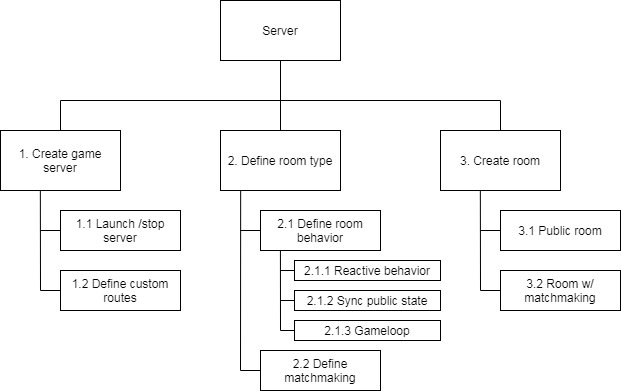
\includegraphics[scale=0.5]{images/2-scoping/server-RBS.png}
   \centering  
   \caption{\textit{RBS for srrver side user requirements.}}
  \label{fig:server-RBS}
\end{figure}

\begin{figure}[H]
  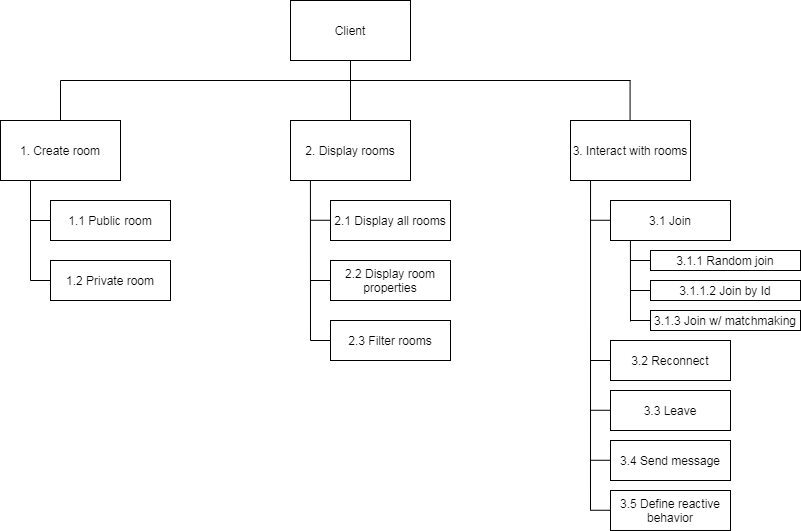
\includegraphics[scale=0.5]{images/2-scoping/client-RBS.png}
   \centering  
   \caption{\textit{RBS for client side user requirements.}}
  \label{fig:client-RBS}
\end{figure}
 
\subsubsection{Use Cases}

We can split use cases in two scenarios about role played by clients: clients that joined a room and clients that didn't. In the first case, the whole system is the context, and it explains high level functionalities of the system. In the latter case, the context is the interaction between a client in a room and such room.

\bigskip
Starting from the first scenery, we have client side and server side programmers that make use of the library as entities interacting with the system.
\\
This is shown in UML use case diagram in figure \ref{fig:system-use_cases}.
\begin{figure}[H]
  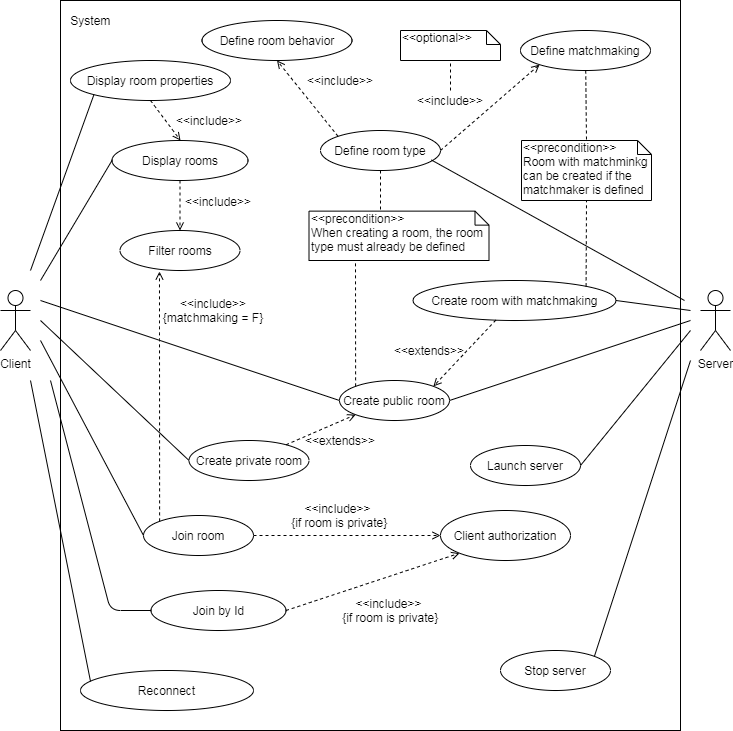
\includegraphics[scale=0.5]{images/2-scoping/system-use_cases.png}
   \centering  
   \caption{\textit{Use case diagram of the system.}}
  \label{fig:system-use_cases}
\end{figure}

\bigskip
About joined room interaction, interacting entities are client side programmer as before for clients, and, a room agent for server, intended as the server side programmer (as before) and/or the room itself with its reactive/proactive behavior defined by the programmer. 
\\
This is shown in UML use case diagram in figure \ref{fig:room-use_cases}.
\begin{figure}[H]
  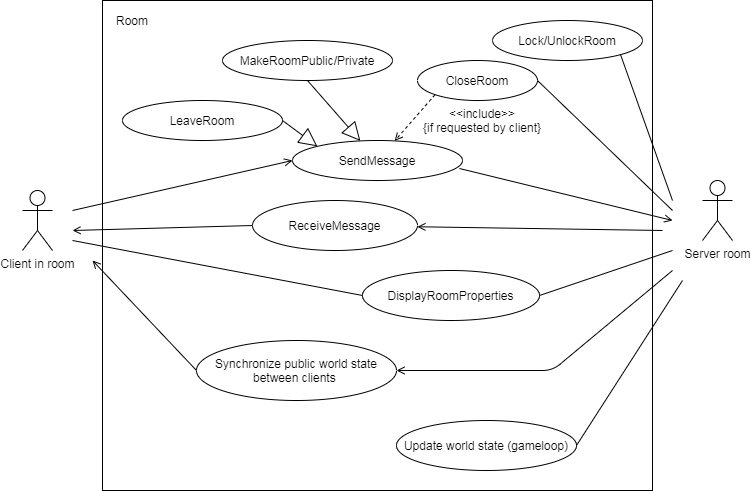
\includegraphics[scale=0.5]{images/2-scoping/room-use_cases.png}
   \centering  
   \caption{\textit{Use case diagram about room interaction scope.}}
  \label{fig:room-use_cases}
\end{figure} 
 
\subsection{Functional Requirements}

Functional requirements, i.e. capabilities that the system should provide, are expressed in table \ref{table:server-f-req} and \ref{table:client-f-req} for server and client respectively.

\begin{center}
  \begin{longtable}{|l|l|} 
    \caption{\textit{Server functional requirements.}} \label{table:server-f-req} \\
  
\hline
ID   &  Specification \\
\hline
\multicolumn{2}{|c|}{} \\
\hline
1         & Create and handle game server \\
1.1       & Launch game server on provided address and port \\
1.2       & Define behavior on server start up \\
1.2       & Suspend/terminate server \\
1.4       & Define behavior on server stop \\
1.5       & Resume suspended server \\
1.6       & Accept user defined routes \\
2         & Define room type \\
2.1       & Define room behavior \\
2.1.1     & Define room reactive behavior \\
2.1.1.1   & Define on create behavior \\
2.1.1.2   & Define on join behavior \\
2.1.1.3   & Define on message received behavior \\
2.1.1.4   & Define on leave behavior \\
2.1.1.5   & Define on close behavior \\
2.1.2     & Define room proactive behavior \\
2.1.2.1   & Handle public state synchronization between clients \\
2.1.2.1.1 & Start state synchronization between clients \\
2.1.2.1.2 & Stop state synchronization between clients \\
2.1.2.1.3 & Resume state synchronization between clients \\
2.1.2.1.4 & Set state synchronization rate\\
2.1.2.2   & Handle room state periodic update (gameloop)  \\ 
2.1.2.2.1 & Start room state periodic update (gameloop) \\
2.1.2.2.2 & Stop room state periodic update (gameloop) \\
2.1.2.2.3 & Resume room state periodic update (gameloop) \\
2.1.2.2.4 & Set state update rate (gameloop) \\
2.2       & Define room properties\\
2.2.1     & Public/private property should be given by default \\
2.2.2     & Room property types could be int, string, boolean, double \\ 
2.3       & Define room state \\
2.4       & Define room type matchmaker \\
2.5       & Ignore multiple room type definitions from second on \\
2.6       & Define custom join constraints depending on room type \\
3         & Lock/unlock room \\
3.1       & Rooms are unlocked by default \\
4         & Close room \\
4.1       & Directly close the room from server \\
4.2       & Expose possibility to close a room for clients \\
4.3       & Notify a client that the room has been closed \\
4.4       & Room auto closing \\
4.4.1     & Allow room auto closing \\
4.4.2     & Auto closing is off by default \\
4.4.3     & Close as auto close timeout expires \\
4.4.4     & Close in front of direct close request even if auto close is on \\
5         & Create room \\
5.1       & Create public room \\
5.2       & Create room with matchmaking \\
5.2.1     & Room with matchmaking should define clients allowed to join \\
5.3       & Rooms create be the server should contain no client at the beginning \\
6        & Display room properties \\
7        & Send messages to clients in a room \\
7.1      & Send a message to one specific client (tell) \\
7.2      & Send a same message to all clients in the room (broadcast) \\
8        & Monitor client liveness \\
8.1      & Heartbeat service (if activated) \\
8.2      & Inactive clients kicking on timeout (if activated) \\
9        & Deny join to room under certain circumstances \\
9.1      & Deny join to private room if no correct password is provided \\
9.2      & Deny join to a locked room \\
9.3      & Deny join to closed room \\
9.4      & Deny join to matchmaking room if not in expected players \\
10        & Allow reconnection for clients to a room \\
10.1      & Allow configuration of a reconnection period length \\
10.2      & Fail reconnection to room under certain circumstances \\
10.2.1    & Fail reconnection to room if client din't previously join the room \\
10.2.2    & Fail reconnection to room if it took too long for the client to reconnect \\
10.2.3    & Reconnection feature is disable by default \\
10.2.3.1  & Allow reconnection timeout length configuration when enabling such feature \\
10.3      & Reconnetion is not considered as a join event \\
11        & Expose possibility to create rooms for clients \\
11.1      & Expose possibility to create public rooms for clients \\
11.2      & Expose possibility to create private rooms for clients \\
12        & Expose possibility to make room public/private for clients \\
\hline

  \end{longtable}
\end{center}

\begin{center}
  \begin{longtable}{|l|l|} 
    \caption{\textit{Client functional requirements.}} \label{table:client-f-req} \\
 
\hline
ID   &  Specification \\
\hline
\multicolumn{2}{|c|}{} \\
\hline
1       & Display rooms, private and public both \\
1.1     & Display all rooms \\
1.2     & Display all rooms of a given type \\
1.3     & Display a room of a given type and with a given Id \\ 
1.4     & Locked rooms should not be displayed \\
1.5     & Matchkaing room should not be displayed \\
1.6     & Rooms can be filtered on their properties \\
1.6.1   & Allowed filter strategies are equal, not equal, grater, lower \\
1.7     & Room Ids should be visible to clients \\
2       & Display all joined rooms, locked and with matchmaking too \\
3       & Create a room \\
3.1     & Create a public room \\
3.2     & Create a private room \\
3.3     & Fail on  create the room if its type is not already defined server side \\
3.4     & Define starting room properties values \\
3.4.1   & Ignore a given room property if such property is not defined in the room \\
4       & Join room \\
4.1     & Join without matchmaking \\
4.1.1   & Random join to public room \\
4.1.1.1 & Allow to specify filters on joinable rooms \\
4.1.2   & Join by room Id \\
4.1.2.1 & When joining by ID, give possibility to provide a password \\
4.1.2.2 & When joining by ID, a provided password will be ignored if the room is public \\
4.1.3   & Auto join a room when creating such room \\
4.2     & Join with matchmaking \\
4.2.1   & Join by Id is not allowed \\
4.2.2   & Filters on rooms with mathcmaking is not allowed \\
5       & Leave a room \\
5.1     & Leaving a room is allowed only if such room has been previously joined \\
6       & Reconnect to room \\
7       & Visualize room properties \\
7.1     & Visualize all properties in a room \\
7.2     & Retrieve value of a single property \\
7.2.1   & Notify error if the specified property does not exist \\
8       & Send messages to a room \\
8.1     & Sending messages to room is enabled once the client joined the room \\
8.2     & When sending amessage to a room, no reply is expected \\
9       & Define reactive behavior to room events \\
9.1     & Define behavior on received message from the room \\
9.2     & Define behavior on state update \\
9.3     & Deifne behavior on room closing \\
9.4     & Definition of reactive behavior is allowed once the client joined the room \\
10      & Close a room \\
11      & Change public/private state of a room \\
11.1    & Make a public room private \\
11.1.1  & When making a public room private, the provision of a password is mandatory \\ 
11.2    & Make a private room public \\
\hline

  \end{longtable}
\end{center}

\newpage

\subsection{Non functional Requirements} 

\begin{itemize}
  \item[\emph{Usability}] The provided library should be easy to use by game developers that are unfamiliar with client-server interaction and newtwork communication protocols.
  \item[\em{Portability}] The provided library should be used in both server and client environments on all major operating systems (i.e Windows, Linux and MacOS).
  \item[\em{Deployment}] The provided library should be easy to deploy, intended as easy to import and make it work on an external project. 
\end{itemize}

\subsection{Implementation Requirements}
The library must be implemented using Scala as main programming language and should adhere to the style definition defined in: https://docs.scala-lang.org/style/
  
 
 

 
\chapter{Development process}

The chosen project management lifecycle (PMLC) is an agile one, in particular Scrum. 
\section{Interactions planning}

In order to end within the given deadline of 60 days, a total of 7 sprints is scheduled. Each sprint is planned to last one week, from Sunday to Sunday. Furthermore, remaining few days after the last sprint are dedicated to the completion of project closing processes, such as system tuning, deploy consummation, documentation refinement and so on.
\\
As Scrum process suggests, each sprint is provided with an initial planning phase and is concluded with review and retrospective meetings. Both current sprint closing and next sprint planning are supposed to be done on Sunday.
\\
Moreover, daily scrum would often be required when tricky features are realized or any non negligible issue is found. Obviously, informal quick message exchange is allowed between team members all day long.
\\
The only exception to such organization is given by the first sprint. Indeed, requirement analysis and system design are predominantly realized at this time, and daily meetings are required to achieve these tasks so that the product backlog, required to plan each sprint from the second on, is produced.
\\
During all the phases of the development process software like Trello and Microsoft Teams are used to support team interaction.


\section{Tasks split and assignment}

Once the product backlog is available, each sprint planning phase produces a sprint backlog containing tasks to complete before such sprint ends. Tasks are chosen from product backlog by priority (importance of a feature in term of business value), considering the estimated size of each task too, so that no sprint is excessively weighted down. Once a task is selected from product backlog, it is split in subtasks by detailing its aspects. Tasks and subtasks sizes are expressed using Fibonacci sequence. 
\\
Once the sprint backlog is built, starting tasks are agreed between all team members, and each one takes charge of a couple of them (2-3 approximatively). The remaining ones are assigned day by day, looking to how the development proceeds. There is no general a priori criteria for task assignment; the only aspect considered, when possible, is to minimize the dependency between tasks assigned to different team members. 
\\
During sprint review, individual work of each member is examined to understand the current situation and to realize if any improvement is needed.

\section{Development tools: Build, Testing, CI}

The building system is automated using the sbt build tool since it is well integrated with Scala.
\\
The development process is not strictly a TDD approach but unit tests on single components and integration tests on use case scenarios are provided to ensure system correctness.  
\\
Moreover,``TravisCI'' combined with ``Github'', is used as continuous integration tool to perform regression tests. Repository is handled with pull requests reviewing flow.
\\
In the end, other plugins/tools used would be ``scalastyle'' and ``scoverage''. The first is used to check code style adherence to specified conventions, meanwhile the latter one helps on quantify tested code and displaying it.

\subsection{Ensuring system portability}

By looking to non functional requirements, portability comes out to be a key aspect. In order to ensure this requirement, Travis is configured to build and test the library upon multiple platforms and OS. In particular:
\begin{itemize}
\item \textbf{OS\footnote{Scala integration with Windows in not available on Travis yet}}: 
  \begin{itemize}
  \item \textit{Linux}
  \item \textit{Osx (MacOS)}
  \end{itemize}
\item \textbf{JDK}:
  \begin{itemize}
  \item \textit{openjdk11}
  \item \textit{openjdk13}
  \item \textit{openjdk-ea (early access)}
  \end{itemize} 
\end{itemize}  

\subsection{Ensuring system deployment easiness}

As described in section \ref{non-fun-req}, the ease of deployment is another key aspect for the library requirements. In order to fulfill this goal, it must be possible to import the library in a project just by using a build tool (e.g. sbt, gradle). This requires the release on a public repository; in this case, ``Maven central'' has been chosen as the designed one.

Two main aspects should be defined to start the process, that is:
\begin{itemize}
  \item \textbf{GroupId}: owners of the library. In this case, an organization named ``com.github.scalaomg'' \footnote{ \url{https://github.com/scalaomg}} has been established.
  \item \textbf{ArtifactId}: name of the library once published. It will be ``scala-omg''.
\end{itemize}

Once the library is be released, it may be found on Maven at: 

\begin{center}
\url{https://search.maven.org/artifact/com.github.scalaomg/scala-omg}.
\end{center}

\bigskip
For example, when using sbt, it can be then imported just by adding 

\begin{center}
\textbf{"com.github.scalaomg" \% "scala-omg" \% "version"}
\end{center}

to library dependencies.































 
\chapter{System architecture}
The library is based on the client-server architectural pattern and his functionalities are indeed split in two distinct modules: 
\begin{itemize}
	\item \textit{Client module} - Provides the main methods to connect and communicate with a game server. In particular allows the client side developer to create rooms (that will be hosted on the server) and to perform operations on them (e.g join, leave, message...).
	\item \textit{Server module} - Internally implements the logic to handle client connections and allows the developer to run a gameserver and define new type of rooms. It also contains all the logic to handle matchmaking requests.
\end{itemize}

However, client and server modules are not fully separated; they share some common concepts like communication protocol used inside websockets or data seriaization utilities to parse data received from the network ecc.. that are grouped in a common packages used by both client and server.

The most important concept that client and server share is anyway the concept of room that is described in detail in the next section. 

\section{Room}

\begin{figure}[H]
	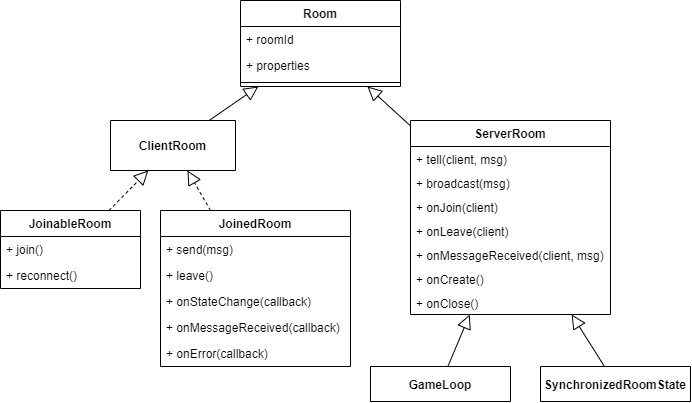
\includegraphics[scale=0.7]{images/3-architecture/room-class-2.png}
	\caption{Room class diagram}
	\label{fig:room_classes}
\end{figure}

At the most abstract level, a room is an entity with a unique id and some shared properties (figure \ref{fig:room_classes}). This fields are accessible both on the client and the server. Then each module extends his own concept of room.

\bigskip
\textit{ServerRoom}
\\
The server room is the one that will be used by the server side developer. It aggregates a list of client and provides the main methods to communicate with them (i.e. tell and broadcast).  This class is meant to be abstract so that the user can extend it and define his own behavior (as expressed in requirement 2.1 of table \ref{table:server-f-req})). Since the developer may want to automatically synchronize the state of the game and have an inner game loop (requirements 2.1.2.1 and 2.1.2.2), there are two extension of the server room: SynchronizedSRoomtate and GameLoop that provide this functionalities.

\bigskip
\textit{ClientRoom}
\\
This is, on the other hand, the room that a client side developer will use. The user can retrieve a list of JoinableRoom from the server; these expose the method \textit{join} that sends a request to the game server to join the given room; a JoinableRoom can also be used to reconnect to a previously left room as express in requirement 5 of Table \ref{table:client-f-req}. Once the joining process to a specific room succedes, a JoinedRoom is created and the user can use it to perform operation on the room (requirements 4, 7, 8 of table \ref{table:client-f-req} ) 

\section{Server architecture}
The main components of the server side architecture are visible in figure \ref{fig:server_classes}. 

\begin{figure}[H]
	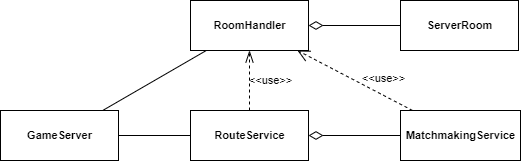
\includegraphics[scale=0.7]{images/3-architecture/server_architecture-classes.png}
	\caption{Server architecture class diagram}
	\label{fig:server_classes}
\end{figure}

\bigskip
\textit{GameServer}
\\
The GameServer is a facade component that is exposed to the user and provides the functionalities to: start and terminate a gameserver; define new type of rooms; create public rooms. To do so, it internally creates two other components that are the RouteService and the RoomHandler.

\bigskip
\textit{RoomHandler}
\\
As the name suggests, the RoomHandler is the handler of the rooms in the application. The purpose of this componenet is to provide functionalities concerning rooms, in particular:
\begin{itemize}
	\item get the list of available rooms
	\item define new type of rooms
	\item create rooms (with and without matchmaking)
	\item query rooms by their properties
	\item connect clients to a specific room
\end{itemize}

\bigskip
\textit{RouteService}
\\
The RouteService defines the routes that the server will listen on and implements all the handlers associated with them. Some routes are fixed since they are used by the library itself and are descibed in table \ref{table:server_routes}; 


\begin{table}[H]
	\begin{tabular}{p{2cm}p{4cm}p{2cm}p{5.5cm}}
		\textbf{Http Method} & \textbf{Path}	  & \textbf{Payload}  & \textbf{Result}                                                            		\\\\
		GET                  & /rooms             & filters           & get all the rooms that match the filters in the payload                        	\\\\
		GET                  & /rooms/:id         & empty             & get the room with the given id                                                 	\\\\
		GET                  & /rooms/:type       & filters           & get all the rooms with the given type (filtered by filters in the payload)     	\\\\
		GET                  & /rooms/:type/:id   & empty             & get the room with the given id searching among rooms of the given type         	\\\\
		POST                 & /rooms/:type       & options           & create a room of the given type with the option passed in the payload          	\\\\
		GET                  & /connection/:id    & websocket request & open a web socket connection with the room that has the given id               	\\\\
		GET                  & /matchmaking/:type & websocket request & open a web socket with the matchmaking service relative to the given room type 	\\\\
	\end{tabular}
	\caption{\label{table:server_routes} \textit{Server basic routes}}
\end{table}

All the routes that requires to perform operation on rooms are managed by the RoomHandler, while routes concerning matchmaking are managed by the appropriate MatchmakingService.


\bigskip
\textit{MatchmakingService}
\\
A MatchmakingService is a component that implements the matchmaking logic expressed in section \ref{server-requirements-gathering} for a given type of room. It use a strategy defined by the user to create client groups and uses a RoomHandler to create the room that will host the match.


\section{Client Architecture}

TODO

\section{Client-Server Interaction}
\subsection{Websockets}









\chapter{Detailed design}

\section{Actor model}

In each module we can detect few different components that may interact in a very complex way. Moreover, each component may own more than one control flow. This could lead to a growth in design complexity and to potential concurrency issues to be solved.
\\
In order to cut those aspects down, components are organized using an actor model. This way, components can be seen as self-contained services that communicate using message passing.
\\
The only drawback is the exposure of the actor model to users that may be forced to think in term of a non trivial programming paradigm. In order to prevent that, library logic and structure is hidden behind an interface layer. This can be achieved just by using a simple facade pattern that permits to mask actor model and message passing by using the solely asynchronous programming, simpler to users the may not know the actor model and more general for users that wouldn't structure their programs using actors.

\section{Room}

Room is one of the main concept of the library, both on server and client perspective; the figure \ref{fig:room_class_diagram} shows its design.
\\
\texttt{Room} is the primary interface that defines a room. A room has a unique identifier and a set of properties. The identifier is an UUID string that can be used by clients to reference a specific room. On the other hand, properties (described in section \ref{room_properties_section}) can be queried to retrieve some useful information exposed by the room.
Both \texttt{ClientRoom} and \texttt{ServerRoom} extend \texttt{BasicRoom}, the one that provides common methods to access properties.
 \\
\texttt{SharedRoom} is the serializable object that is passed through the network to share room information between clients and server.
\\
The following sections provide a more detailed description of client and server specializations of the room concept, focusing on \texttt{ClientRoom} and \texttt{ServerRoom} classes.



\begin{figure}
	\centering
	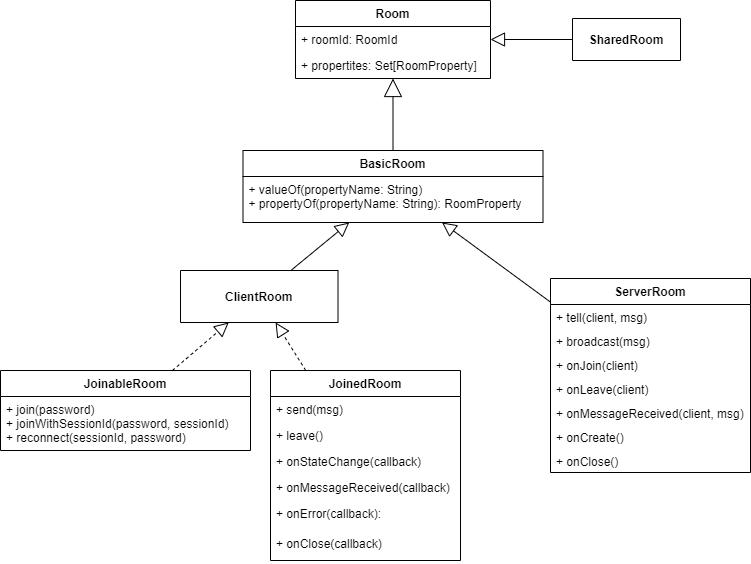
\includegraphics[scale=0.5]{images/4-design/room-class.png}
	\caption{Room class diagram}
	\label{fig:room_class_diagram}
\end{figure}

\subsection{ServerRoom}
\begin{figure}
	\centering
	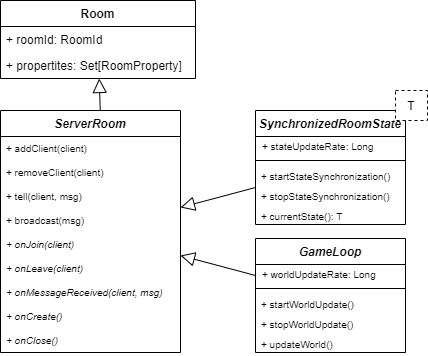
\includegraphics[scale=0.5]{images/4-design/server-room.png}
	\caption{Server room class diagram}
	\label{fig:server_room_class_diagram}
\end{figure}

\texttt{ServerRoom} is a trait that encapsulates the concept of room used server-side; as we see in figure \ref{fig:server_room_class_diagram}, it extends the \texttt{Room} trait by adding methods to manage clients (add, remove, tell and broadcast) and by defining abstract handlers for room events. These handlers are the ones that the developer must implement to define his own type of room.
\\
Few extensions are provided to enhance its functionalities, in particular:

\begin{itemize}
    \item \texttt{MatchmakingSupport}: it gives the developer access to the matchmaking groups created by the matchmaking service associated with this room.
	\item \texttt{PrivateRoomSupport}: it manages private rooms by allowing the possibility to set a password to the room in order to prevent undesired accesses.
	\item \texttt{RoomLockingSupport}: it enables lock and unlock functionalities to the room.
	\item \texttt{ReconnectionSupport}: it allows clients reconnection to the room.
	\item \texttt{SynchronizedRoomState}: it permits to synchronize the public state of the room between clients using a period of \texttt{stateUpdateRate}.
	\item \texttt{GameLoop}: it permits to update the room state using a period of \texttt{stateUpdateRate}.
\end{itemize}

Differently from the others, \texttt{SynchronizedRoomState} and \texttt{GameLoop} are optionals and can be included by the developer at will.

The first one is a trait generic in the type of the state that needs to be synchronized to clients; all methods are implemented, except for \texttt{currentState} that must be defined by the user. This method should return the new world to be synchronized between the clients.

The latter is also a trait and requires to define \texttt{updateWorld}, a method that is assigned to update the room using a given logic.

\subsection{ClientRoom}

\texttt{ClientRoom} is the client-side representation of the room.
This concept has been then specialized in two further concepts: ``Joinable'' and ``Joined''.
This separation was made to provide the developer a consistent access to room functionalities. Indeed, by using this structure, it is not possible to execute unauthorized operations on rooms. For example, leaving a room that wasn't joined yet or joining a room that is already joined.

\bigskip
\texttt{JoinableRoom} extends a basic \texttt{ClientRoom} and adds join and reconnect accessing protocols.


\bigskip
\texttt{JoinedRoom} extends the \texttt{ClientRoom} trait too and enables the definition of callbacks on room events: message received, state changed, room closing or communication error.
Furthermore, it also exposes methods to send messages and leave the room.
\\
A client is provided with a \textit{sessionId} that identifies the joining of the client to the room.
This can be used, for example, in the reconnection process in order to recognize the client on the server.


\subsection{Properties and Filters}  \label{room_properties_section}
UML class diagram in figure \ref{fig:property-class} shows the detailed architecture of room properties and filters.

\bigskip
\textit{Basic room properties}
\\
Each property (\texttt{BasicRoomProperty}) owns a name and a value.
\\
Values, since they can be of four types (server requirements 2.2.2), are modeled as classes that extend a common trait \texttt{RoomPropertyValue}. This trait wraps a ``real'' value of type \texttt{Int}, \texttt{Double}, \texttt{Boolean} or \texttt{String}.
\\
Each property value exposes two main features: the real value wrapped by the class and a method that compares such value to another one of the same type (e.g. compare the \texttt{Int} value wrapped by the class to another given \texttt{Int}); this is useful since different type of values may define different comparing logics.
Moreover, there is also a static factory that permits to create a property value from a given first class value (if possible).

\bigskip
\textit{Filters}
\\
By looking to client requirement 1.6.1, there are four available filter strategies. Similarly to property values, they are hidden behind a common trait \texttt{FilterStrategy}. Such trait defines a name for the strategy and an evaluation predicate that permits to apply the strategy to two values. The evaluation result expresses if the filtering defined by the strategy is satisfied.

\bigskip
Since library usability is a core aspect, a simple DSL language is created in order to easily manage filters.
\\
\texttt{BasicRoomProperty} functionalities are extended to include filters by using mixins. This way, filter strategies can be directly called by the property itself.
\\
A \texttt{FilterOption} is something that contains the name of the property to be filtered, the strategy to be uses and a value the property should be compared to. It exposes an utility method to concatenate two \texttt{FilterOption} too.
\\
A \texttt{FilterOptions} is a wrapper around a set of \texttt{FilterOption}; this is useful when talking about DSL since it permits to define static factories (\texttt{empty}, \texttt{just}) and utility methods such as concatenation (\texttt{and}) and union (\texttt{++}).

\bigskip
\textit{Design notes / implementation directives}
\begin{itemize}
\item Before on choosing this design, few different options have been analyzed, and this has been decided to be the most feasible one. The only lack that can be detected is on the value getter of \texttt{RoomPropertyValue}. Indeed, it is absent in the class instance itself, and it is only available through the static method \texttt{valueOf}.
\item Notice that, in order to encourage library usability, the value wrapper can be made be transparent to final users thanks to implicit conversions that can be defined in Scala.
\end{itemize}
\begin{figure}[H]
	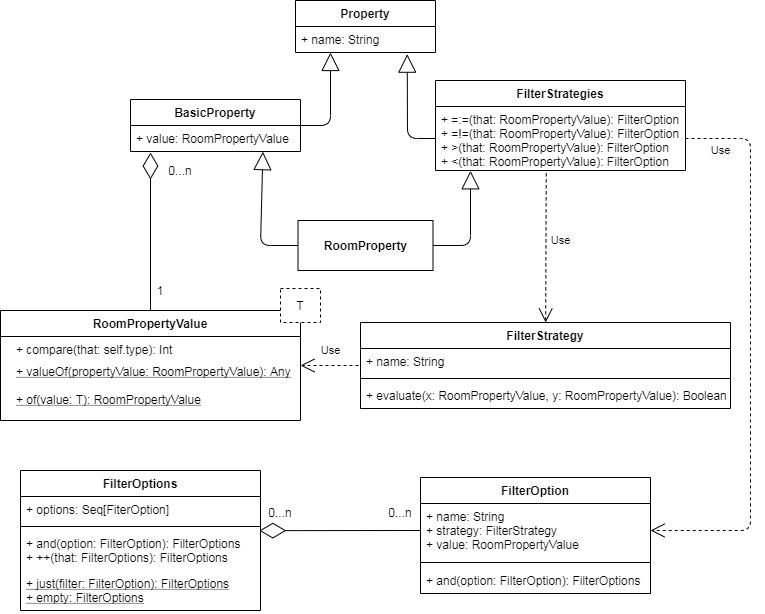
\includegraphics[scale=0.45]{images/4-design/property_and_filters-class.png}
	\caption{Properties and filters class diagram.}
	\label{fig:property-class}
\end{figure}

\newpage

\section{Server}
Class diagram in figure \ref{fig:server_class_diagram} describes in detail the server architecture by describing its main functionalities and by showing its components interactions.
\begin{figure}[h]
	\hspace*{-1.1in}
	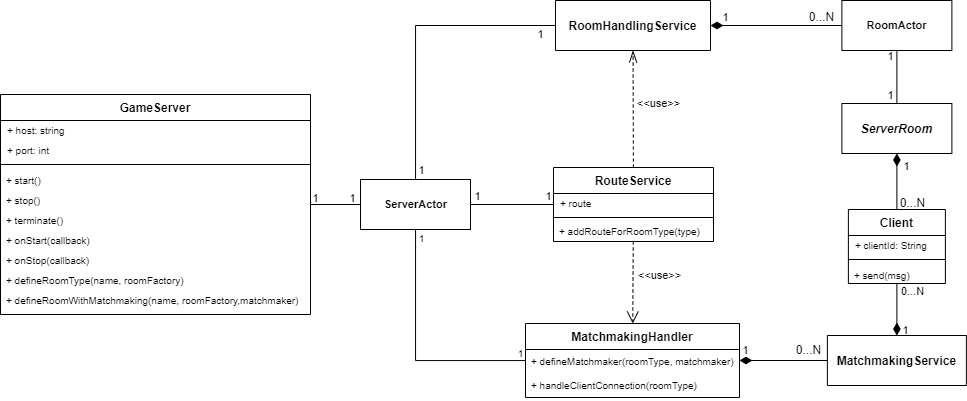
\includegraphics[scale=0.55]{images/4-design/server_class.png}
	\caption{Server class diagram}
	\label{fig:server_class_diagram}
\end{figure}

\textit{Game server and routing service}
\\
The \texttt{GameServer} class is the facade interface that is exposed to the developer. It internally creates a \texttt{ServerActor} that is the entity acting as the real server listening for clients requests. This actor creates a \texttt{RouteService} object that is used to know which routes to use and how to handle requests; it also allows to dynamically define new room types that will be used by the server.

The \texttt{ServerActor} also uses a \texttt{RoomHandlingService} actor to create and define rooms from the server itself. The same actor is used by the \texttt{RouteService}.

\bigskip
\textit{Rooms and room handling service}
\\
As we described for the server architecture in section \ref{sec:server_arch}, the purpose of the \texttt{RoomHandlingService} is to manage the active rooms in the application. Specifically, it doesn't directly create rooms; instead, it creates \texttt{RoomActor}(s), namely actors used as ``wrappers'' for \texttt{ServerRoom}(s) to avoid concurrency issues and to semplify the overall system design. This is required since more than one client can interact with a single room at the same time and so, in order to avoid race conditions, clients communicate with \texttt{RoomActor}(s) that process messages sequentially. Each actor is in charge of notifying clients' actions to the room it is associated with.

\bigskip
\textit{Client}
\\
Each \texttt{ServerRoom} is linked to an actor and keeps track of connected clients (\texttt{Client} class server-side). Clients are uniquely identified by their Id and expose a \texttt{send} method that allows to send messages to them. It is important to notice that each room has its own view of clients: the same client connected to different rooms will have a different Id in each of them.

\bigskip
\textit{Matchmaking}
\\
Each matchmaking service has an internal actor assigned to handle all incoming requests. This actor needs to know which \texttt{Client}(s) are waiting for the match start.
Since clients may ask for matchmaking, the \texttt{RouteService} uses a \texttt{MatchmakingHandler} to redirect those requests to the right \texttt{MatchmakingService} actor.
Moreover, when defining a new room type with enabled matchmaking, the server will demand the \texttt{RouteService} to add the right route and to spawn the associated \texttt{MatchmakingService}.


\section{Client}
Class diagram in figure \ref{fig:client_class_diagram} describes the detailed client architecture.

\bigskip
\textit{Core client}
\\
The \texttt{Client} class is the main access point to its api. It's a facade that exposes client's primary functionalities while hiding the underlying actor model.
\\
The main logic is internally handled by the \texttt{CoreClient} actor. It exploits an \texttt{HttpService} actor to make http requests to the game server when getting or creating rooms.
\\
Moreover, it keeps track of currently joined rooms. The list, once created, is kept updated by interacting with the \texttt{ClientRoomActor}'s associated with each room.

\bigskip
\textit{Client room}
\\
The \texttt{ClientRoomActor} is an actor that handles the socket connection with the server side room. 
It's spawned when joining a room, and it's killed when the room is left or closed. It notifies the \texttt{CoreClient} when the associated room is left, joined or closed so that the list of joined rooms can be updated.
\\
In the end, the callbacks specified by the user, i.e. the ones that define the client side room reactive behavior, are handled by this actor internally.

\bigskip
\textit{Matchmaking}
\\
The \texttt{ClientMatchmaker} can be used to access the matchmaking functionality. It exposes methods to join or leave matchmaking queues for given room types. It keeps track of active matchmaking connections so that it is always possible to leave queues without waiting the matchmaking process to be completed.
\\
A \texttt{MatchmakingActor} is spawned when a new matchmaking request is performed.
This actor opens a websocket connection with the server side matchmaker and notifies the client after the the joinin operation on the room created by the matchmaking service. This actor is killed when the matchmaking process completes or the relative matchmaking queue is left.
\begin{figure}[H]
	\hspace*{-1in}
	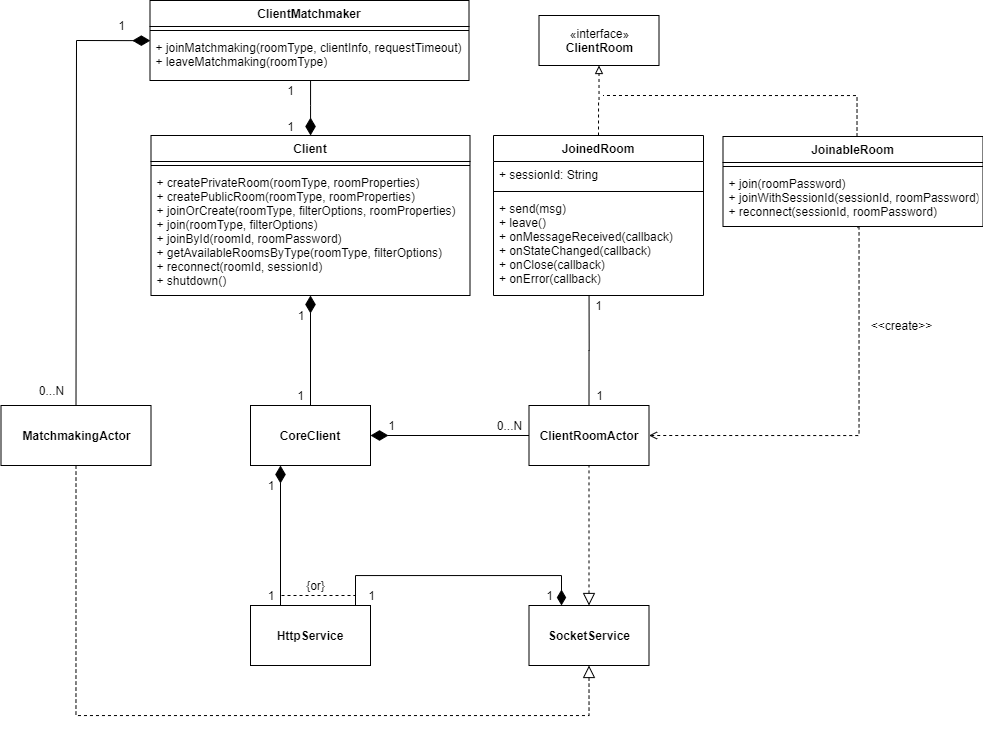
\includegraphics[scale=0.55]{images/4-design/client_class.png}
	\caption{Client class diagram}
	\label{fig:client_class_diagram}
\end{figure}

\section{Communication}\label{sec:communication_design}


\subsection{Json Serialization}
For Request-Response interaction (described in section 3.4), Json format has been used for client requests and server responses both. \texttt{RoomJsonSupport} class provides json-formatted serialization capabilities for all entities that are exchanged at this stage of client-server interaction, in particular:
\begin{itemize}
	\item \texttt{SharedRoom} objects and related (e.g. roomId).
	\item Room properties and related/derivatives (e.g. set of properties, property value).
	\item Room filters and related/derivates (e.g. filter strategies, \texttt{FilterOptions}).
\end{itemize}

\subsection{Websockets}
\begin{figure}[h]
	\hspace*{-0.5in}
	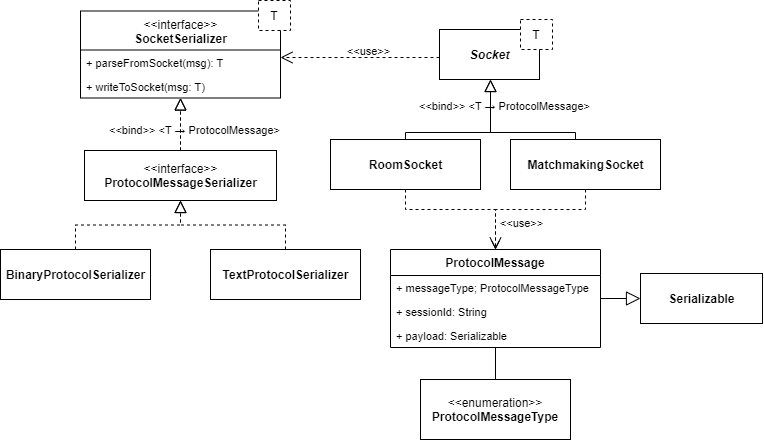
\includegraphics[scale=0.6]{images/4-design/communication_protocol.png}
	\caption{Websocket class diagram}
	\label{fig:websocket_communication_design}
\end{figure}
Regarding websockets, a class diagram describing the main classes is shown in figure \ref{fig:websocket_communication_design}.
The \texttt{Socket} abstract class provides the main functionalities for a socket communication and allows to define the configuration for the connection (heartbeat rate, idle timeout). It is generic in T where T represents the type of messages sent through that socket . Two concrete implementations are provided for this class:
\begin{itemize}
	\item \texttt{RoomSocket}: used for the communication between client and rooms.
	\item \texttt{MatchmakingSocket}: used for the communication between client and matchmaking services.
\end{itemize}
They are \texttt{Socket} both where the generic type T is a \texttt{ProtocolMessage}. Indeed, this is the class that defines the communication protocol between client and server. It uses a structure made up of three fields to describe a message sent through a socket:
\begin{itemize}
	\item \textit{MessageType} \\
	Used to identify the type of message that the client or the server want to send. The list of the possible message types is defined in the \texttt{ProtocolMessageType} enumeration.
	\item \textit{SessionId} \\
	Used to identify the client that is sending the message through the socket. When a websocket connection is established between client and server, a unique Id is generated; the client must always use the same sessionId to send messages through that socket.
	\item \textit{Payload} \\
	An optional payload that can be carried with the massage. This is, for example, the field used to store messages when a client sends a message to the server through the usage of \texttt{sendMessage} method on the client room. It must be \texttt{Serializable} since it will eventually be serialized to be sent to the server.
\end{itemize}

In order for a \texttt{Socket} object to send and receive data, it must be able to serialize and deserialize messages that pass through it. It uses for this purpose a \texttt{SocketSerializer} that has two methods: \texttt{parsefromSocket} and \texttt{writeToSocket}. This class is generic in T that is the type of messages that needs to be read and written.

Since \texttt{RoomSocket} and \texttt{MatchmakingSocket} need to handle \texttt{ProtocolMessage}(s), a \texttt{ProtocolMessageSerializer} interface specifically defines a serializer for protocol messages. Two types of serializers are implemented: \texttt{BinaryProtoclSerializer} and \texttt{TextProtocolSerializer}. The first one serializes protocol messages as binary data, the latter, instead, as text messages.
 
Two different implementations are present because Json format may be also used for socket communication by exploting the \texttt{TextProtocolSerializer}. However, the binary representation improves performance and usability both (a developer just needs to extend \texttt{java.io.Serializable} vs. create a Json parser using \texttt{spray.sjon.RootJsonFormat}). Hence, at the moment, the binary representation is the used one, and the Json format is kept just because of its usefulness in testing purposes.

\bigskip
Sequence diagram in figure \ref{fig:create_room_seq} shows an example of full interaction between client and server. Specifically, it represents a client request about the creation of a new room.

\begin{figure}
	\hspace*{-1in}
	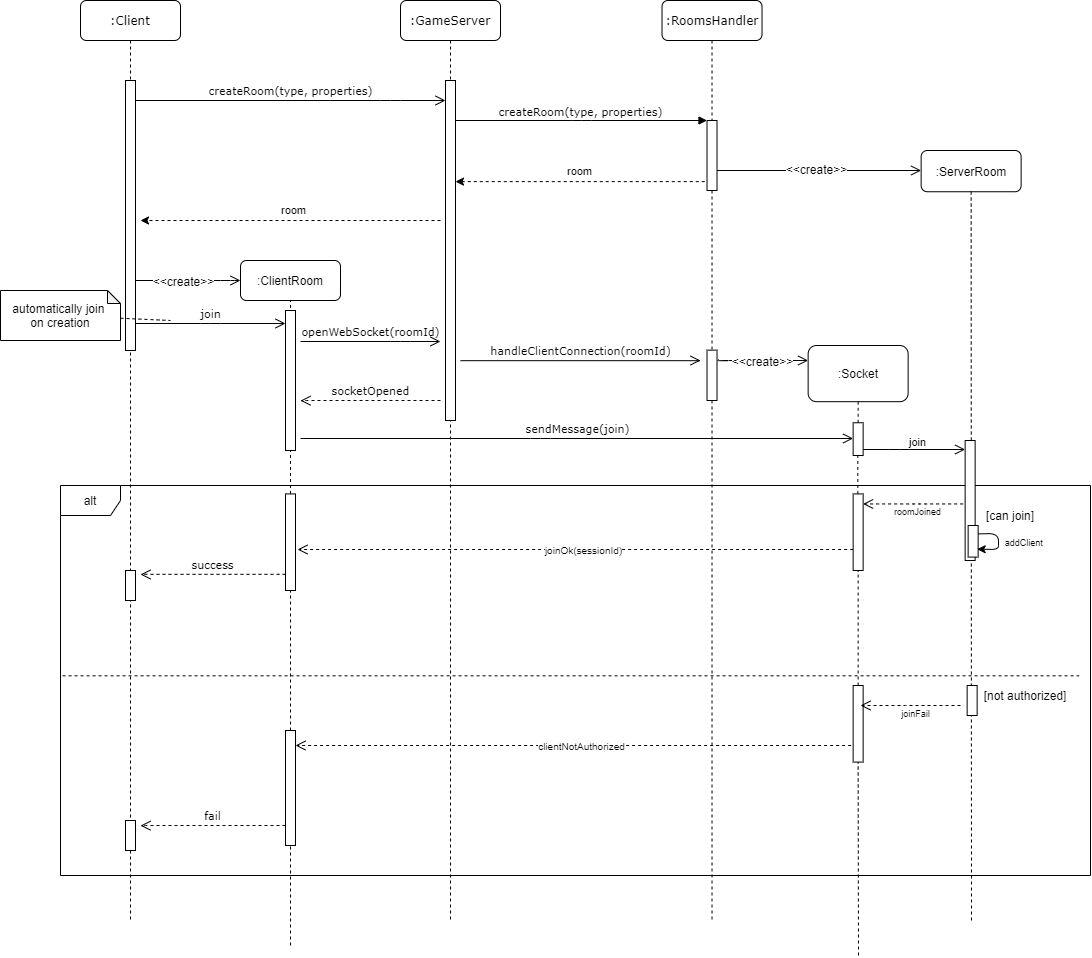
\includegraphics[scale=0.5]{images/4-design/create_room_seq.png}
	\caption{Example of a client-server interaction upon a 'create room' request}
	\label{fig:create_room_seq}
\end{figure}
\input{5-implementation.tex}
\chapter{Retrospective}

\section{Development description in detail}

\subsection{Sprint 0}
\subsubsection{Report}
During the first meeting the product backlog of the project and the product items were defined. Each product item was associated with an estimate of his development effort.
The organizational structure of the project was also defined. We discussed tools and development environments to support continuous integration.
An initial analysis and design process was carried out in order to define the main entities and how to manage their interactions.
It was therefore decided to internally use an approach base on actor, which however is transparent to the user (developer). 
We decided to rely upon akka-core library and akka-http library. 
In the end it was decided to carry out the development of clients and server in parallel in ordeer to have a working core in the shortest time. This core would be extended incrementally during the project lifetime.

\subsubsection{Retrospective}

???






\subsection{Sprint 1}
\subsubsection{Report}
The goal of this first sprint was to define the main client and server interfaces and reach a minimal working system that allows:
\begin{itemize}
	\item game server execution 
	\item room types definition
	\item client requests to create rooms.
\end{itemize}
This goal was completed successfully. 

The task effort concerning the creation of a game server based on an existsing server was underestimated; this lead us to re-think some decision that were made upon server creation. The result is that is possible for the user to specify some external routes, this will be handled by the game server if they don't conflict with existing routes used internally. 
However, it is not possibile to attach the game server to an existing one.





\subsubsection{Retrospective}
The team was able to effectivly use continuous integration and project managemenet tools settled in the firts meeting  and complete all tasks.
A problem that arised was that some scalastyle rules were too strict and tests were failing with no good reason. We decided then to disable such rules in further development.

\subsection{Sprint 2}
\subsubsection{Report}
The amount of work spent on this sprint was certainly greater than the previous one.
Indeed during this week some of the main features of the library about clients and rooms have been developed.
Tasks regarding web socket support was underestimated so it was not fully completed during this sprint. Given the amount of work spent on this task some other were left behind and were not fully completed too.
The task of creating a room with custom options was not completed due to the lack of communication about who was the volunteer of that task.
Uncompleted tasks will be completed in the next sprint.

The interaction between client and rooms required the definition of an ad hoc protocol to manage the messages used internally by the library. This introduced some dependecies between client and server tasks causing some slowdown in the development process.



\subsubsection{Retrospective}
Even if the estimated effort for this sprint was high, the fact that the team was not able to complete all task require some further considerations.
First, it's important to better define the work in advance. For example we should consider splitting tricky tasks in multiple sub-tasks when needed.
Furthermore the communication between the team should be increased even during the week.
This could help solving problems that arises during the development in advance, before reaching the end of the week.


\subsection{Sprint 3}
\subsubsection{Report}

In this week tasks pending from the previous sprint were completed.

During the implementation of the automatic state update we decided to use binary serialization instead of json serialization. Json serialization required the user to define his own parsers while binary serialization allowed a more generic and simple approach.

Since the work done in the previous weeks contained the core functionalities of the library, we were able to implement a simple online multiplayer game.
The game is Rock-Paper-Scissor. 
The purpose of implementing this application was to verify that the code produced so far was robust and usable in a simple manner both client and server side.
The final code is also a good example on how to use the library and his basic functionalities.


\subsubsection{Retrospective}
This time the tasks were all completed. 
Anyway the lack of documentation and diagrams relative to some common concepts led to different integration issues  between code written by different team members. Sometimes ad hoc refactoring was needed to keep high quality software throughout the development.
More attention must be paid to the documentation process, particulary the one concerning important aspects of the library. 

During the week were added to the test suite a subset of unpredictable tests.
They were immediatly fixed after their discovery, within the end of the sprint.




\subsection{Sprint 4}
\subsubsection{Report}
In this sprint was implemeneted 'MoneyGrabber', a game that takes advantage of the most advanced features of the library, such as the automatic update of the state of the world and the management of rooms with multiple players.
It was therefore possible to verify the actual versatility of the library showing a further and more complex example of use in a real context.
All tasks were completed ahead of time.
Probably we should have considered the addition of some more tasks to the backlog during the previous sprint review. By the way the remaining time of the sprint was used by the whole team to improve the existing code quility and produce some more detailed documentation.



\subsubsection{Retrospective}

???






\section{Sprint 5}

\subsubsection{Report}

\subsubsection{Retrospective}

\section{Sprint 6}

\subsubsection{Report}

\subsubsection{Retrospective}


\section{Final comments}	
	
\backmatter	

\end{document}